% self defined colors for colored code (can add more colors)
\definecolor{green}{rgb}{0.1,0.5,0.2} % rgb defined between 0 and 1
\definecolor{blue}{rgb}{0,0.3,0.7}
\definecolor{purple}{rgb}{0.7,0,0.7}
\definecolor{gray}{rgb}{0.5,0.5,0.5}
\definecolor{codeorange}{rgb}{0.9,0.3,0}

% writing code in the document as list
% can be changed, add changed version before your code (possible to have multiple versions within one doc)
\lstset{ 
  basicstyle=\ttfamily\UseRawInputEncoding\small,
  extendedchars=true, % lets you use non-ASCII characters; for 8-bits encodings only, does not work with UTF-8
  breaklines=true,                 
  escapeinside={\%*}{*)}, % if you want to add LaTeX within your code
  keepspaces=true,
  morekeywords={*,...}, % if you want to add more keywords
  showstringspaces=false,          
  tabsize=2, % sets default tabsize to 2 spaces
  numbersep=5pt, % how far the line-numbers are from the code
  numbers=left,                   
  numberstyle=\tiny\color{gray},
  stringstyle=\color{purple},
  commentstyle=\color{gray},
  keywordstyle=\color{blue},
  identifierstyle=\color{codeorange}
}

%=================================================================
%                           Start Document
%=================================================================
\section{Dataset utilizzato}
\lhead{Dataset} % section header

\subsection{Descrizione del dataset}
Il dataset scelto per il progetto è \textit{egoFacebook}, disponibile su \textbf{SNAP} (Stanford Network Analysis Platform): una libreria attiva dal 2004 che tutt’oggi è in crescita organica grazie all’attività di ricerca nell’analisi di grandi reti sociali e informative. In generale, la libreria offre dataset di reti di vario genere: dai dati relativi a Facebook, Twitter, fino a Wikipedia.

Questo dataset consiste in 'circles' (o 'liste di amici') provenienti da diversi utenti Facebook. I dati sono stati prelevati utilizzando un'applicazione di Facebook ad oggi non più disponibile a causa di un cambio di politiche di Meta, azienda proprietaria del social network. Dataset simili attualmente possono essere generati utilizzando l'API Graph di Facebook, il metodo principale tramite cui le app possono leggere e scrivere nel social graph di Facebook. È possibile ottenere l'accesso all'API Graph di Facebook creando un'applicazione sulla sezione \textit{Facebook for Developers} di Facebook ed ottenere una API Key, da utilizzare poi nell'applicazione per inviare richieste all'API Graph tramite HTTP GET o POST.


\subsection{Caratteristiche del dataset}

Il dataset utilizzato presenta al proprio intero 4 reti, ognuna rappresentante la lista di amici di uno specifico utente Facebook che, per motivi di privacy, è reso anonimo. Le reti presentano una struttura abbastanza simile, tutte presentano una componente gigante che comprende la maggior parte dei nodi (per ogni rete, la componente gigante contiene almeno il 97\% dei nodi.). Le reti differiscono nel numero dei nodi; la rete più piccola contiene appena 150 nodi, la più grande contiene 1034 nodi. La rete più piccola, rappresentante la rete di amicizie dell'individuo anonimo 414, contiene la percentuale più alta di triangoli. La percentuale di triangoli è stata calcolata come il rapporto tra i triangoli presenti nel grafo e i possibili triangoli del grafo $\binom{|V|}{3}$. Seguono ulteriori dettagli sulle reti nella seguente tabella:

\begin{table}[htbp]
\centering
\begin{tabularx}{\linewidth}{l *{6}{>{\centering\arraybackslash}X}} % Usa tabularx con larghezza della linea
\toprule
\textbf{Rete} & \textbf{Nodi} & \textbf{Edges} & \textbf{Size CG} & \textbf{CG (\%)} & \textbf{Triangoli} & \textbf{Tr. (\%)} \\
\midrule
Rete 414 & 150 & 1693 & 148 & 98.67\% & 10618 & 1.93\% \\
Rete 348 & 224 & 3192 & 224 & 100\% & 23503 & 1.27\% \\
Rete 0 & 333 & 2519 & 324 & 97.30\% & 10740 & 0.18\% \\
Rete 107 & 1034 & 26749 & 1034 & 100\% & 420329 & 0.23\% \\
\bottomrule
\end{tabularx}
\caption{Dati delle reti nel dataset}
\label{tab:network_data}
\end{table}

\newpage
\subsection{Visualizzazione del dataset}

\begin{figure}[htbp]
  \centering
  \begin{subfigure}[b]{0.4\textwidth}
    \centering
    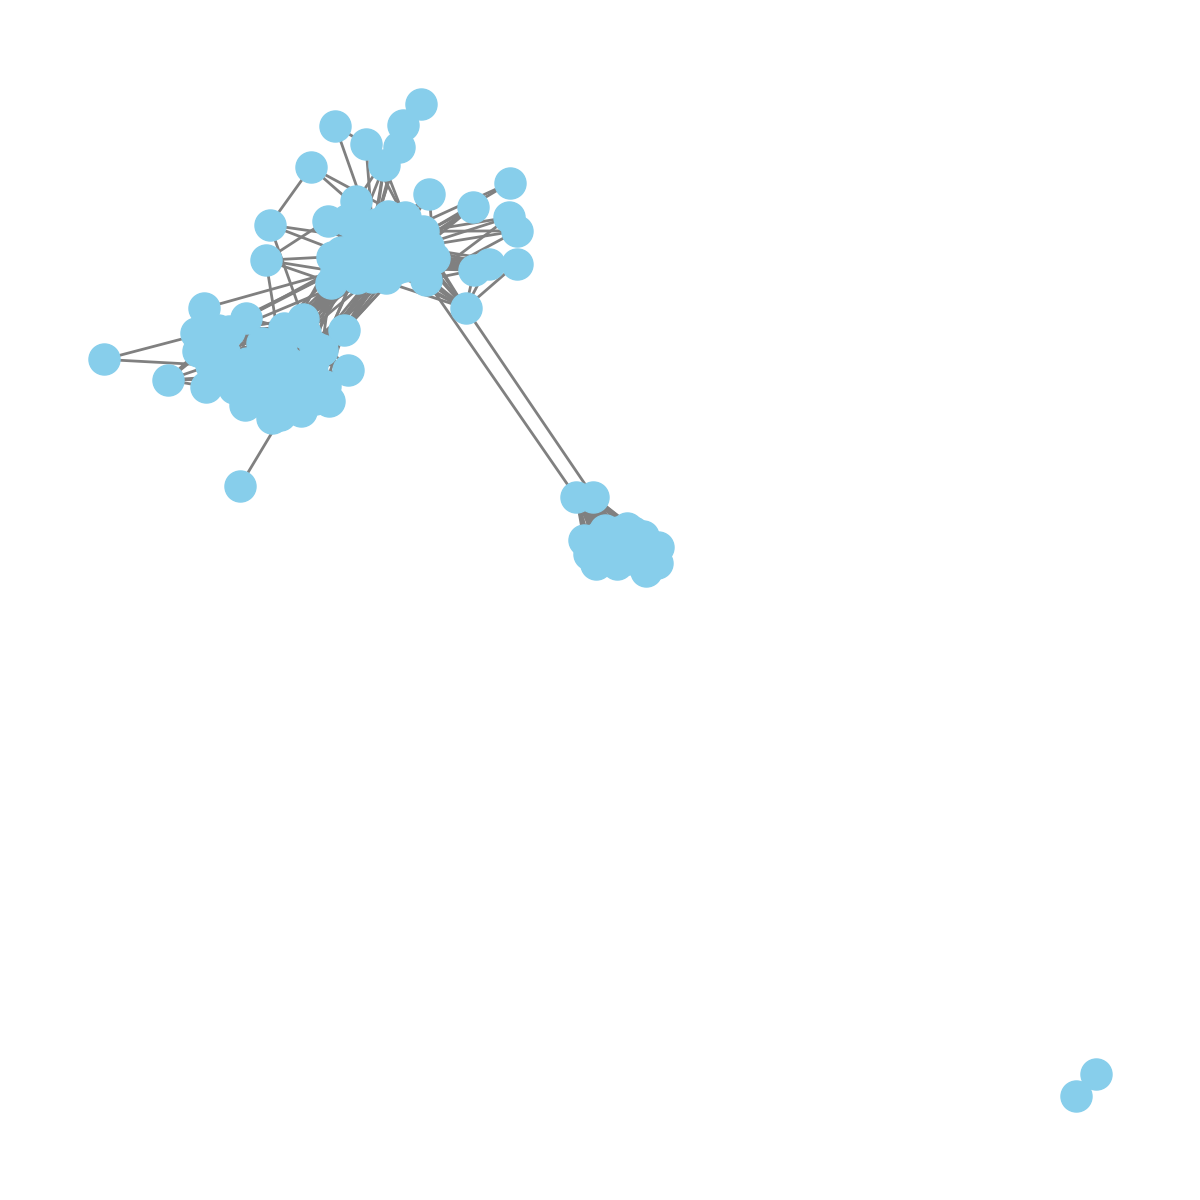
\includegraphics[width=\textwidth]{images/414.png}
    \caption{Rete 414}
    \label{fig:sub1}
  \end{subfigure}
  \hfill
  \begin{subfigure}[b]{0.4\textwidth}
    \centering
    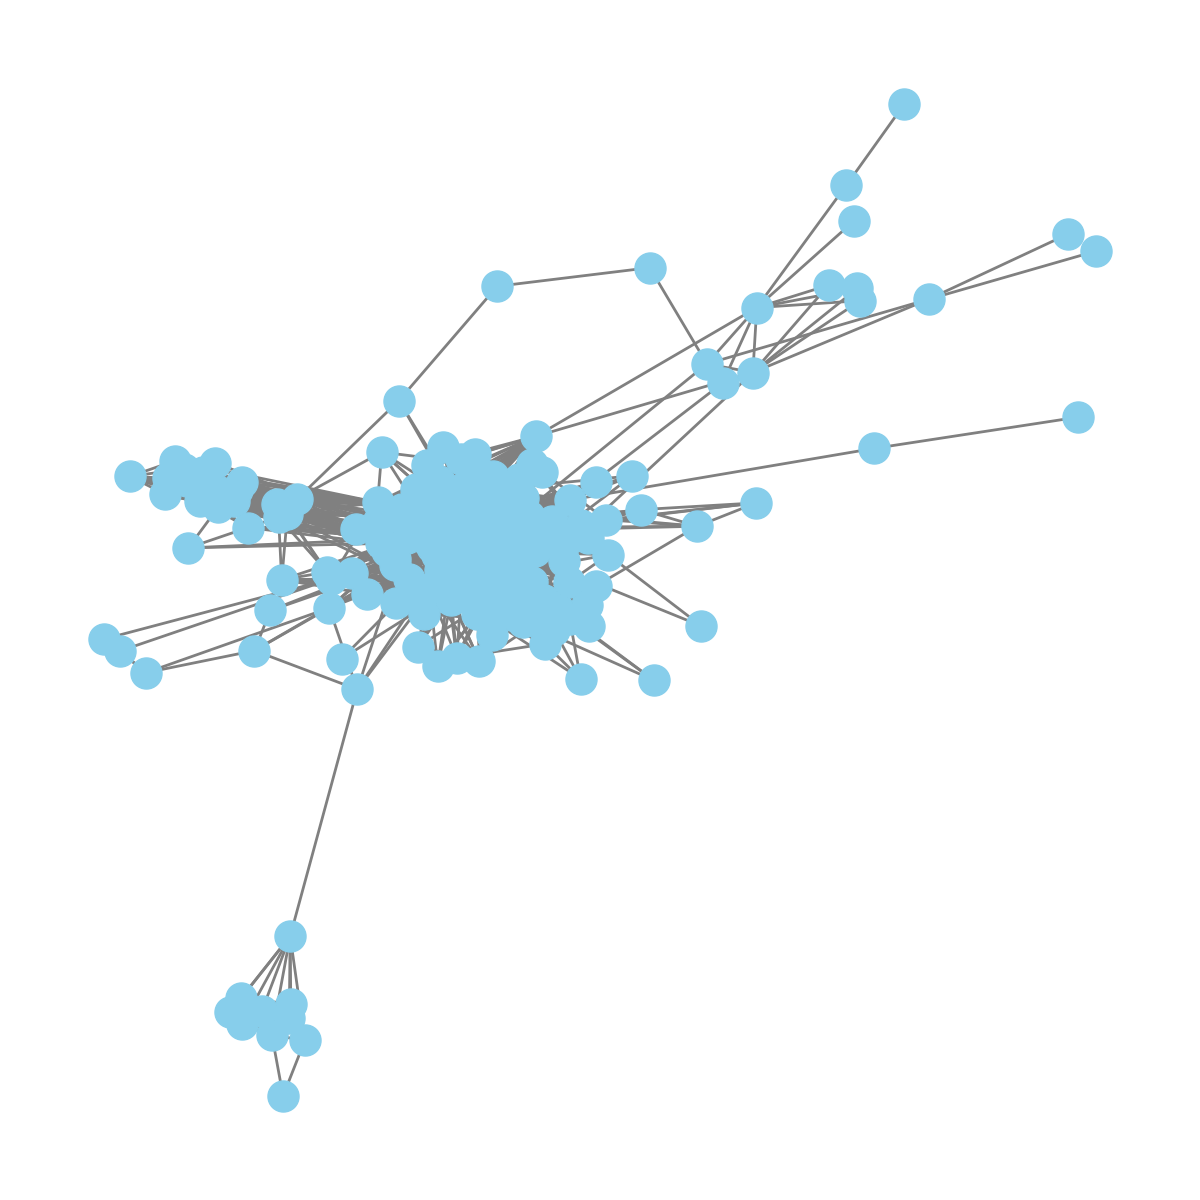
\includegraphics[width=\textwidth]{images/348.png}
    \caption{Rete 348}
    \label{fig:sub2}
  \end{subfigure}
  \vskip\baselineskip
  \begin{subfigure}[b]{0.4\textwidth}
    \centering
    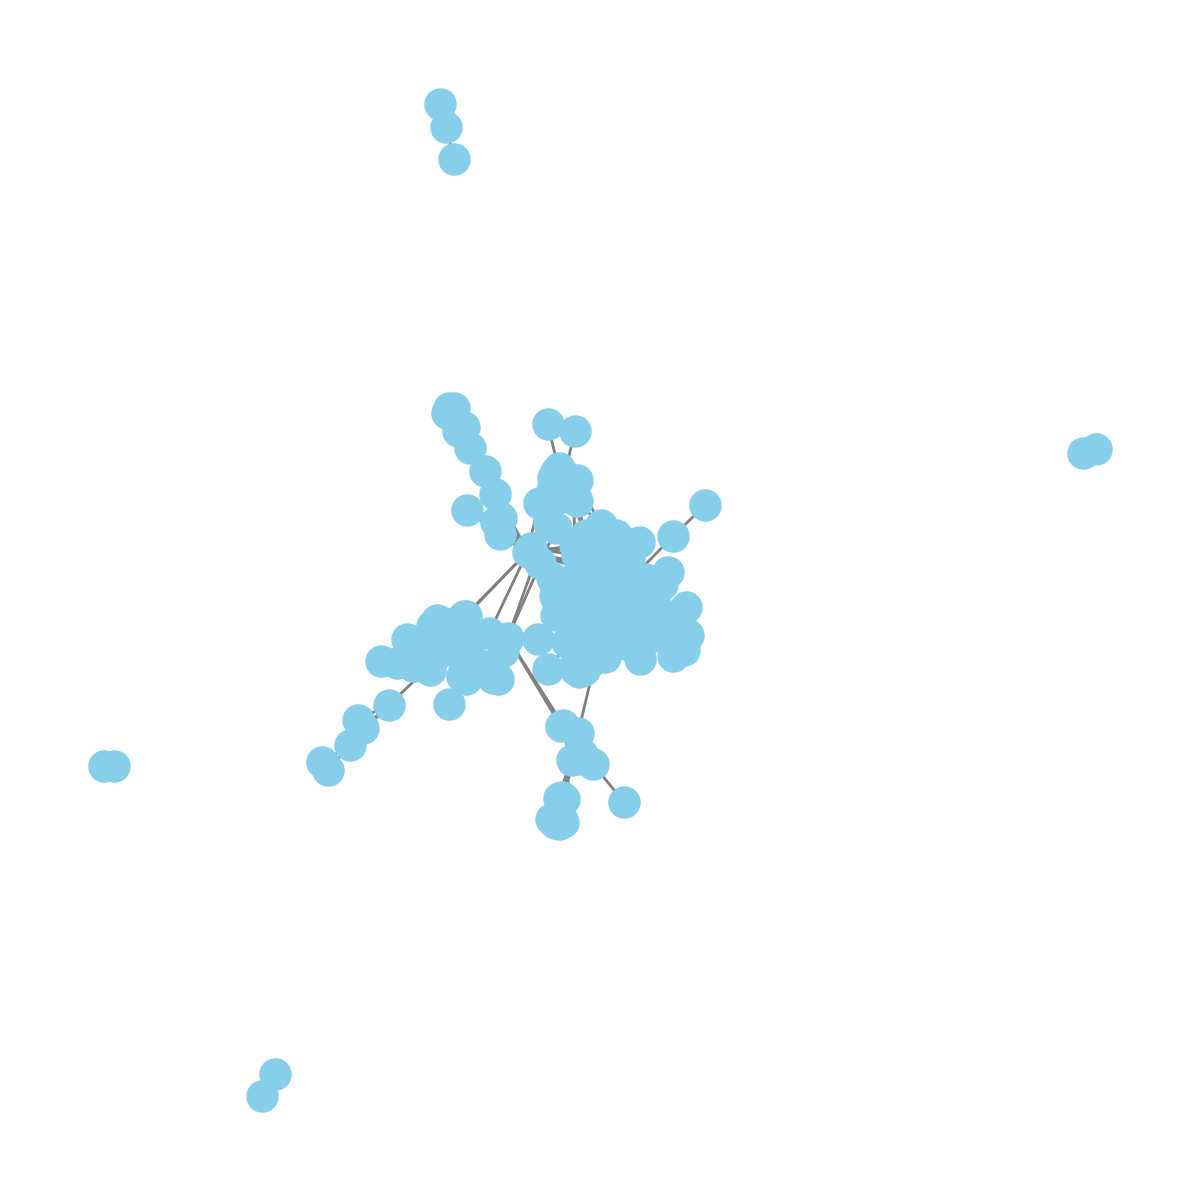
\includegraphics[width=\textwidth]{images/0.png}
    \caption{Rete 0}
    \label{fig:sub3}
  \end{subfigure}
  \hfill
  \begin{subfigure}[b]{0.4\textwidth}
    \centering
    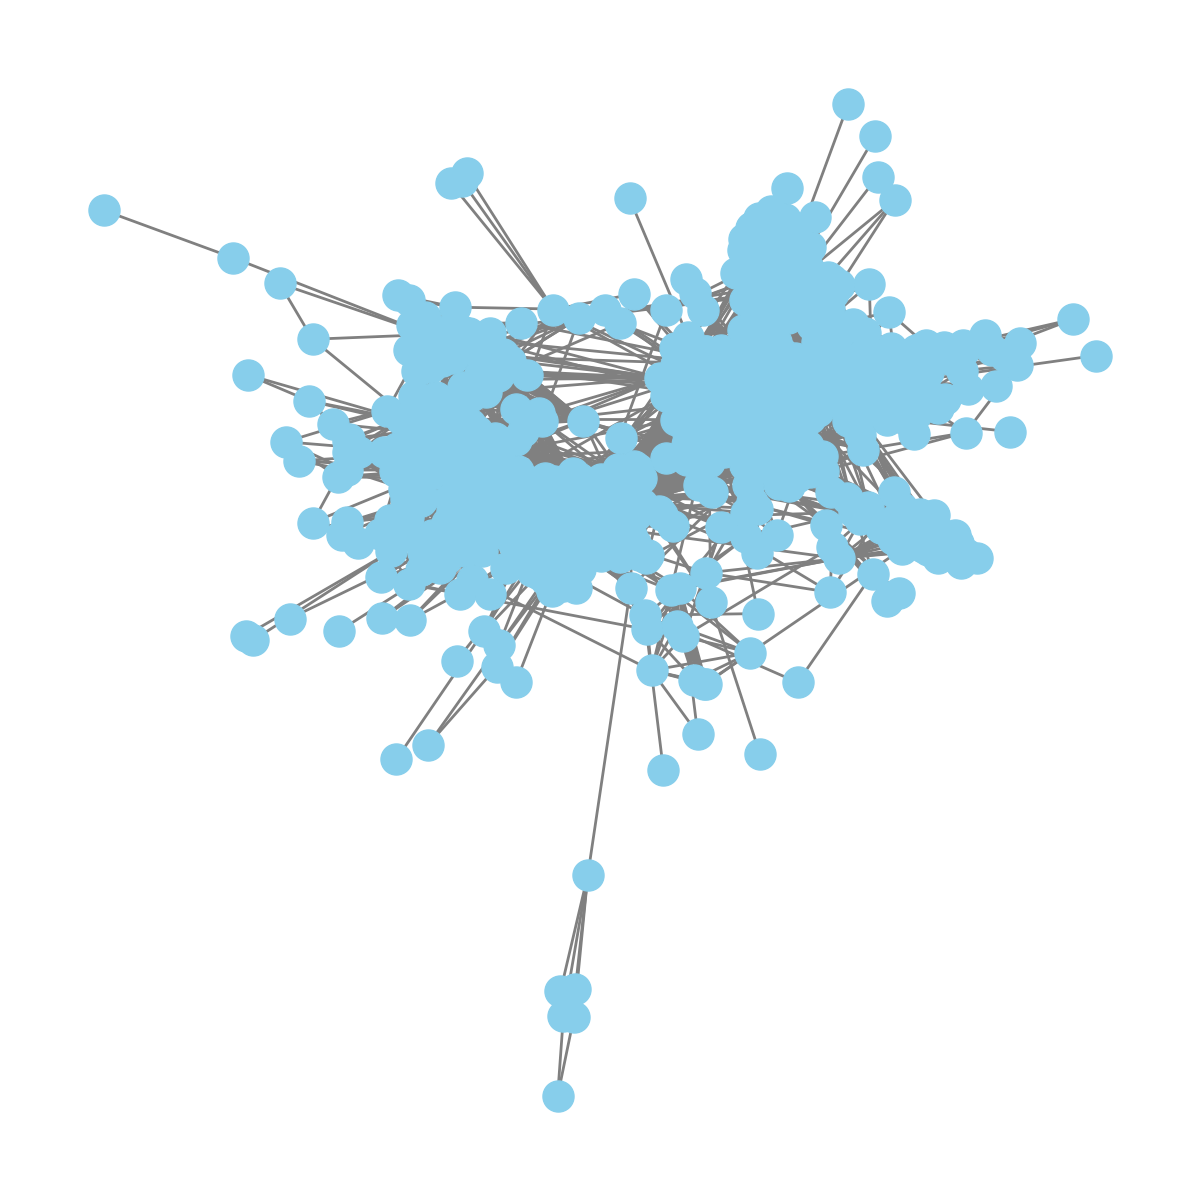
\includegraphics[width=\textwidth]{images/107.png}
    \caption{Rete 107}
    \label{fig:sub4}
  \end{subfigure}
  \label{fig:grid}
\end{figure}

Le immagini sono state generate con la libreria \textbf{matplotlib} di Python. Per favorire la visualizzazione è stato usato come algoritmo di posizionamento dei nodi lo Spring Layout della libreria \textbf{networkx}. Le reti presentano pressochè strutture simili anche graficamente. Dove la componente gigante non comprende la totalità dei nodi è possibili osservare pochi nodi sparsi ed isolati, lontani dal centro.

\subsection{Scelta della rete}

Per le nostre sperimentazioni è stata scelta la \textbf{rete 348}, il miglior compromesso tra dimensione e complessità; la scelta di questa specifica rete è giustificata dai tempi di esecuzione \textit{accettabili} per l'ottenimento dei risultati finali da valutare e commentare relativi alle nostre sperimentazioni.